\section{Preliminary}
\label{saber:sec:preliminary}

\subsection{Video Generation Models}
\label{saber:sec:video_model}
Video generation models~\citep{hong2022cogvideo, yang2024cogvideox, kong2024hunyuanvideo, hacohen2024ltx, wan2025wan} have achieved remarkable progress and gained broad attention.
Among these, the Wan Video series (\eg, Wan2.1~\citep{wan2025wan}) is one of the most popular open-source frameworks.
Our method builds on the Wan2.1-14B model~\citep{wan2025wan}, which consists of a variational autoencoder (VAE)~\citep{kingma2013auto}, a transformer backbone~\citep{vaswani2017attention, peebles2023scalable} and a text encoder (\ie, umt5-xxl~\citep{chung2023unimax}).
%
The VAE encodes videos into temporally and spatially compressed latents ${\mathbf{z}_{0}}$ and decodes them back to pixel space, reducing token count and computation.
% The text prompt and reference image are encoded by the text encoder,image encoder and VAE to form the condition $\mathbf{c}$ that guides the diffusion model.
%
% The text encoder encodes the text prompt $\mathbf{P}$ into a text embedding $\mathbf{z}_\mathbf{P}$, while the image encoder encodes the first-frame image $\mathbf{I}$ into an image embedding $\mathbf{z}_\mathbf{I}$.
% To enable image-conditioned control, Wan2.1 adopts a transformer input composed of three parts: the noisy latent $\mathbf{z}_\mathbf{t}$ (randomly sampled Gaussian noise $\epsilon$ added to ${\mathbf{z}_\mathbf{0}}$ at timestep $\mathbf{t}$, the mask input $\mathbf{z}_\mathbf{m}$ ($0$ for non-reference, $1$ for reference frames), and the condition input $\mathbf{z}_\mathbf{cond}$ (the first frame $\mathbf{I}$ concatenated with zero frames and encoded by the VAE).
% These components are concatenated along the channel dimension to form $\mathbf{z}_\mathbf{cat}$, which is then fed into the transformer.
% The transformer takes $\mathbf{z}_\mathbf{cat}$, $\mathbf{z}_\mathbf{P}$, $\mathbf{z}_\mathbf{I}$, and the timestep $\mathbf{t}$ as inputs.
% In each transformer block, $\mathbf{z}_\mathbf{cat}$ first undergoes spatiotemporal self-attention, then interacts with the text embedding $\mathbf{z}_\mathbf{P}$ and image embedding $\mathbf{z}_\mathbf{I}$ through cross-attention, followed by an feed-forward network (FFN).
% The timestep $\mathbf{t}$ is processed by a time-conditioned multi-layer perceptron (MLP) and injected into the intermediate latents to provide diffusion time step conditioning.
% After several blocks, the transformer outputs $\mathbf{z}_\mathbf{t-1}$.
%
Wan2.1 trains the diffusion model $\Psi$ using Flow Matching (FM)~\citep{lipman2022flow}, where the forward process linearly interpolates between data and noise.
For a time step $t \in [0, 1]$, Gaussian noise $\epsilon \sim \mathcal{N}(0, I)$ is added to $\mathbf{z}_{0}$ to obtain $\mathbf{z}_{t}$, following $\mathbf{z}_{t} = (1 - t) \mathbf{z}_{0} + t \epsilon$.
The model is optimized to predict the target velocity with the following objective:
\begin{align}
\label{eq:loss}
    \mathcal{L}_\text{FM} = \mathbb{E}_{\mathbf{z}_{0}, \epsilon, t, c} \left[\left\|(\mathbf{z}_{0} - \epsilon)  - \Psi_\theta ( \mathbf{z}_{t}, t, c)\right\|_{2}^{2} \right],
\end{align}
where $\theta$ denotes the learnable parameters of the diffusion model $\Psi$, and $c$ represents the condition features derived from the given text prompt and reference images.

\subsection{Task Definition and Notations}
\label{saber:sec:task_define}
% reference images: $\{ \mathbf{I}_{k} \}_{k=1}^{K}$
% generated video: $\{ \mathbf{I}_{f} \}_{f=1}^{F}$
Given $K$ reference images $\{ \mathbf{I}_{k} \in \mathbb{R}^{H_{k} \times W_{k} \times 3}\}_{k=1}^{K}$ and a text prompt $\mathbf{P}$, the reference-to-video method generates a video $\{ \mathbf{I}_{f} \in \mathbb{R}^{H \times W \times 3} \}_{f=1}^{F}$ whose subjects preserve the identities and appearances of those in the reference images while following the instructions in text prompt $\mathbf{P}$.
Here, $H_{k}$ and $W_{k}$ denote the height and width of the corresponding $k$-th reference image $\mathbf{I}_{k}$, while $F$, $H$, and $W$ represent the number of frames, height, and width of the generated video.


\section{Method}
\label{saber:sec:method}

Our goal is to train a diffusion model $\Psi_\theta$ capable of generating videos $\{ \mathbf{I}_{f} \}_{f=1}^{F}$ that preserve the identity and appearance of subjects in the given reference images $\{ \mathbf{I}_{k} \}_{k=1}^{K}$ while following the provided text prompt $\mathbf{P}$. 
Previous methods~\citep{liu2025phantom, jiang2025vace, hu2025hunyuancustom, hu2025polyvivid, li2025bindweave} rely on reference image-video-text triplets, which are costly and hard to scale.
In contrast, Saber achieves R2V capabilities using only video-text pairs, the same data paradigm used for T2V and I2V training.

% say why this data construction pipeline is cost and complex. cite related papers, and point out the hardest problem.
Our core idea of Saber is to simulate the R2V task by replacing the explicitly collected reference images with randomly masked frames during training.
This masked training strategy is supported by two key components to enhance robustness and visual quality: i) a series of mask augmentations designed to mitigate copy-paste artifacts, and ii) a tailored attention mechanism that guides the model to focus on relevant reference features.

We first introduce the construction of masked frames in Sec.~\ref{saber:sec:masked_frames}, including mask generation and augmentation.
Next, we present the model's architecture design in Sec.~\ref{saber:sec:model_design}, detailing the input format and transformer-based attention mechanism.
Finally, Sec.~\ref{saber:sec:inference} describes the zero-shot R2V inference process.


\subsection{Masked Frames as Reference}
\label{saber:sec:masked_frames}

A standard R2V model learns to extract identity and appearance features from reference images $\{ \mathbf{I}_k \}_{k=1}^{K}$ and inject them into the generated video $\{ \mathbf{I}_{f} \}_{f=1}^{F}$.
% We observe that clear subject boundaries in reference images are unnecessary during training, as randomly masked frames can serve the same purpose.
% Moreover, existing R2V datasets~\citep{yuan2025opens2v, chen2025phantom} mainly contain humans and common objects, limiting subject diversity and hindering the model’s ability to generalize.
% In contrast, our randomly masked frames introduce richer and more diverse visual information, allowing the model to learn better subject integration and achieve stronger generalization.
However, existing R2V datasets~\citep{yuan2025opens2v, chen2025phantom} mainly consist of humans and common objects, leading to limited subject diversity and poor generalization.
To address this, instead of relying on pre-collected reference images, we use randomly masked frames as dynamic substitutes during training. 
This strategy naturally introduces highly diverse reference samples, allowing the model to learn more effective subject integration and achieve stronger generalization.

% masked frames: $\{ \hat{\mathbf{I}}_\mathbf{k} \}_{\mathbf{k}=1}^{\mathbf{K}}$
As shown in Fig.~\ref{saber:fig:mask_frames}, for each $k$-th reference image $\mathbf{I}_k$ randomly sampled from the video, we first use a \textbf{mask generator} to produce a binary mask $\mathbf{M}_{k} \in \{0, 1\}^{H \times W}$.
To mitigate the copy-paste issue~\citep{liu2025phantom} in R2V tasks, we perform \textbf{mask augmentation} to disrupt spatial correspondence between the masked references and their corresponding video frames.
Specifically, we apply an identical set of spatial augmentations to both $\mathbf{I}_k$ and $\mathbf{M}_k$, producing $\bar{\mathbf{I}}_{k}$ and $\bar{\mathbf{M}}_{k}$.
The masked frame $\hat{\mathbf{I}_{k}}$ is then obtained as $\hat{\mathbf{I}}_{k} = \bar{\mathbf{I}}_{k} \odot \bar{\mathbf{M}}_{k}$.
This process is repeated to create the full set of $K$ masked frames $\{ \hat{\mathbf{I}}_{k} \}_{k=1}^{K}$ that serve as the reference condition.

\begin{figure*}[t]
    \centering
    % \fbox{\rule{0pt}{2in} \rule{1.0\linewidth}{0pt}}
    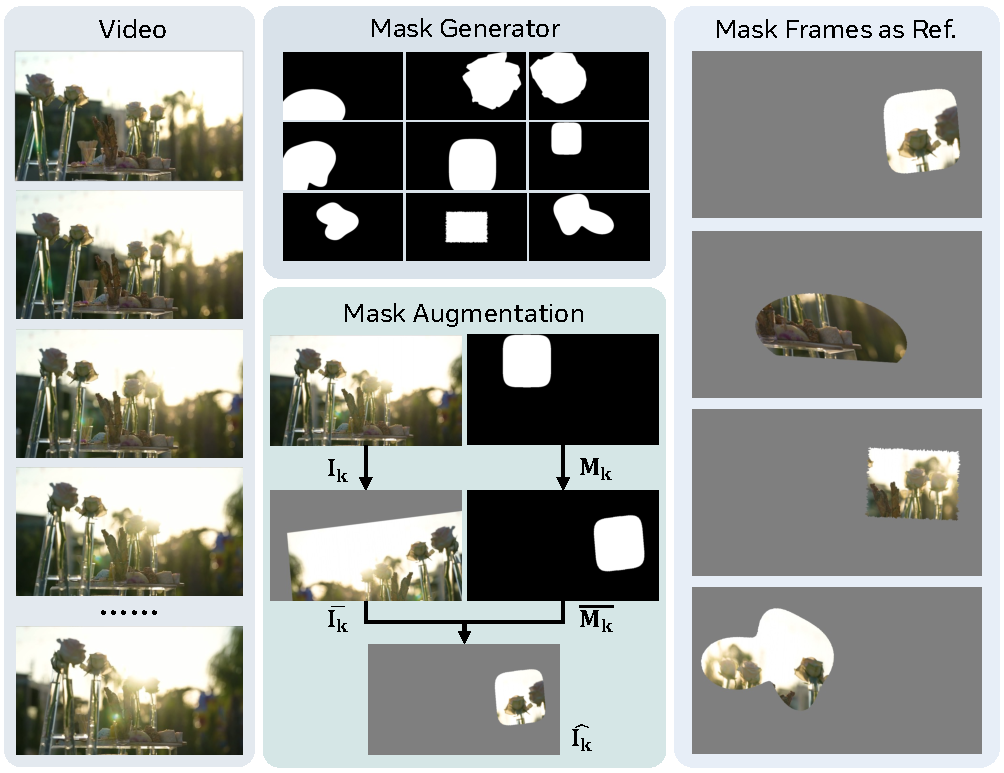
\includegraphics[width=0.6\linewidth]{Chapter7/Figures/mask_frames.pdf}
    \caption{
    Masked reference generation.
    Given a video, the mask generator produces diverse random masks, which are then applied to each randomly sampled video frame with mask augmentation.
    }
    \label{saber:fig:mask_frames}
\end{figure*}


\noindent \textbf{Mask Generator.}
We randomly select one mask type from predefined shape categories (\eg, ellipse, Fourier blob, convex/\allowbreak concave polygon, \etc) to generate a binary mask $\mathbf{M} \in \{ 0, 1 \}^{H \times W}$ with a target foreground area ratio $r \in [r_\text{min}, r_\text{max}]$.
Specifically, we first randomly select a foreground center.
To ensure that the generated mask meets the desired foreground area ratio $r$, we define a continuous scale parameter for each shape category, where the mask's foreground area increases monotonically with the scale.
A bisection search over the scale is then performed to satisfy the area ratio constraint.
When pixel discretization prevents an exact match, small topology-preserving adjustments are applied: ``growth'' dilates background boundary pixels, while ``shrinkage'' erases background boundary pixels.
This design ensures controllable foreground area ratios while maintaining diversity in mask shapes.
Several mask examples are illustrated in Fig.~\ref{saber:fig:mask_frames} Top.

\noindent \textbf{Mask Augmentation.}
We apply random affine transformations, including rotation, scaling, shear, translation, and optional horizontal flip, to both the image $\mathbf{I}_{k}$ and its mask $\mathbf{M}_{k}$, ensuring the masked region remains fully inside the frame.
Transformation parameters are uniformly sampled within predefined ranges and validated to avoid boundary overflow.
The same affine transformation is applied to the image and mask using bilinear and nearest-neighbor interpolation, respectively.

The reference code of the mask generator and augmentation are provided in the supplementary materials.



\subsection{Model Design}
\label{saber:sec:model_design}

After obtaining the masked frames $\{ \hat{\mathbf{I}}_{k} \}_{k=1}^{K}$ as reference images, we detail our model design for the R2V task.
We adopt a simple yet effective \textbf{input format} by concatenating reference images along the temporal dimension at the end of the target video frames in latent space.
This allows the model to manage the interaction between the target video latents and reference latents through the \textbf{attention mechanism} in each transformer block.

\noindent \textbf{Input Format.}
Given a video-text pair $\{ \mathbf{I}_{f} \}_{f=1}^{F}$ and $\mathbf{P}$, and the masked frames $\{ \hat{\mathbf{I}}_{k} \}_{k=1}^{K}$ as reference images, we use the VAE to encode the video from pixel space into latent space, obtaining $\mathbf{z}_{0} = \{ \mathbf{z}_{\hat{f}} \in \mathbb{R}^{h \times w \times d} \}_{\hat{f}=1}^{\hat{F}}$.
Here, $\hat{F} = \lfloor(F - 1) / 4\rfloor + 1$, where $4$ is the temporal compression ratio of the Wan2.1 VAE~\citep{wan2025wan}, $h$, $w$, and $d$ denote the height, width, and feature dimension of the video latent, respectively.
We obtain $\mathbf{z}_{t}$ with time step $t$ following Sec.~\ref{saber:sec:video_model}.
For the reference images, we individually encode each $\hat{\mathbf{I}}_{k}$ using the VAE to obtain $\mathbf{z}_\text{ref} = \{ \mathbf{z}_{k} \in \mathbb{R}^{h \times w \times d} \}_{k=1}^{K}$.
Accordingly, each $\mathbf{M}_{k}$ is resized to match the latent space resolution, producing $\mathbf{m}_\text{ref} = \{ \mathbf{m}_{k} \in \{0,1\}^{h \times w \times 4} \}_{k=1}^{K}$, where $0$ indicates non-reference and $1$ indicates reference region.
The transformer input $\mathbf{z}_\text{in}$ is defined as in Eq.~\ref{eq:input_format}:
\begin{equation}
\label{eq:input_format}
\mathbf{z}_{\text{in}} = \mathsf{cat}
\begin{bmatrix}
    \mathsf{cat}[ & \mathbf{z}_{t}         & \mathbf{z}_\text{ref} & ]_\text{temporal} \\
    \mathsf{cat}[ & \mathbf{m}_\text{zero} & \mathbf{m}_\text{ref} & ]_\text{temporal} \\
    \mathsf{cat}[ & \mathbf{z}_\text{zero} & \mathbf{z}_\text{ref} & ]_\text{temporal}
\end{bmatrix}_\text{channel},
\end{equation}
where $\mathsf{cat}[\cdot]_\text{temporal}$ and $\mathsf{cat}[\cdot]_\text{channel}$ denote concatenation along the temporal and channel dimensions, respectively. $\mathbf{z}_\text{zero}$ is the VAE-encoded latent of a zero-value video, and $\mathbf{m}_\text{zero}$ is an all-zero mask, both shaped to match the temporal dimensions of the video part.
Note that $\mathbf{z}_\text{ref}$ remains noise-free to preserve accurate conditioning.


\begin{figure*}[t]
    \centering
    % \fbox{\rule{0pt}{2in} \rule{1.0\linewidth}{0pt}}
    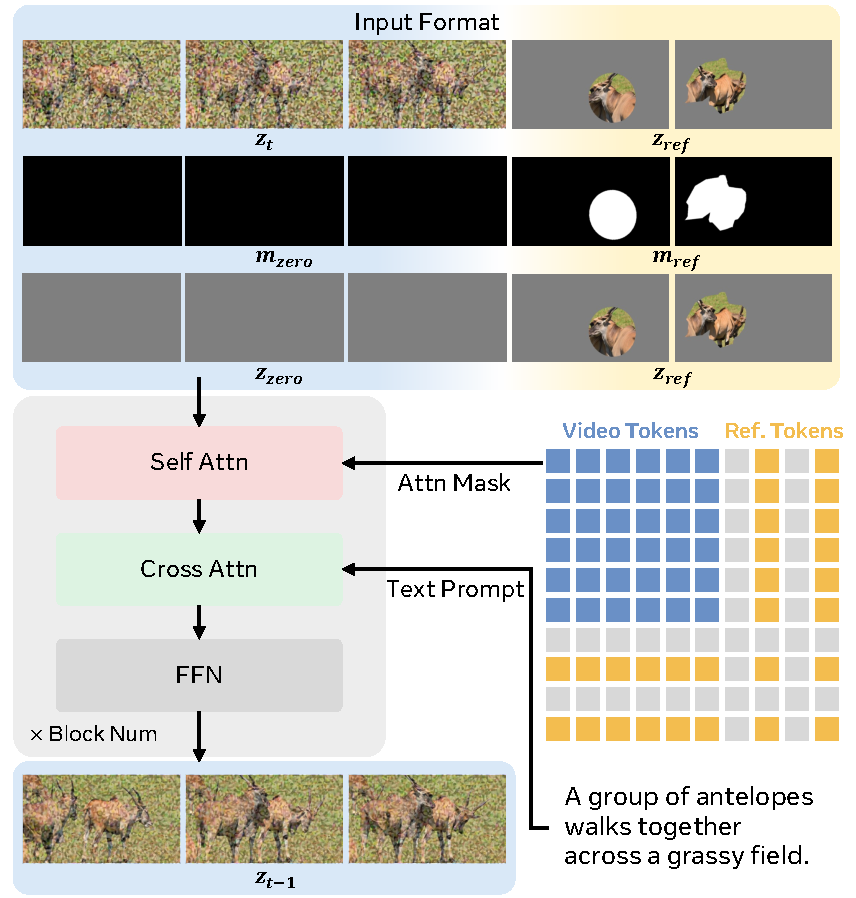
\includegraphics[width=0.6\linewidth]{Chapter7/Figures/model_design.pdf}
    \caption{
    Model design overview.
    Masked frames serve as reference images and are concatenated to the video tokens in latent space.
    Self-attention enables interaction between video and reference tokens under the attention mask, while cross-attention incorporates text guidance for semantic alignment.
    The VAE, text encoder, and timestep components are omitted for clarity.
    }
    \label{saber:fig:model_design}
\end{figure*}


\noindent \textbf{Attention Mechanism.}
After obtaining the transformer input $\mathbf{z}_\text{in}$, we encode the text prompt $\mathbf{P}$ into text features $\mathbf{z}_\text{P}$ and jointly feed them, along with the time step $t$, into the transformer.
Each transformer block consists of a self-attention, cross-attention, and feed-forward (FFN) modules.

In self-attention, the video and reference parts of $\mathbf{z}_\text{in}$ interact with each other.
To avoid attending to non-reference regions, each $\mathbf{M}_{k}$ is resized to match the flattened latent shape to form an attention mask, where video tokens are bi-directionally attended, and only valid reference regions are attended in the reference part.

The self-attention output is then passed to the cross-attention module to interact with $\mathbf{z}_\text{P}$.
Here, video tokens are guided by the text prompt, while reference tokens learn their semantic alignment, enabling the integration of reference image information under textual constraints.
The FFN module refines the results, with the time step $t$ injected into the latents for the control of the time step.
After multiple transformer blocks, the transformer model outputs the predicted latent $\mathbf{z}_{t-1}$.
The model design is shown in Fig.~\ref{saber:fig:model_design}.
% Note that patchify and unpatchify layers are applied at the input and output to flatten and reconstruct the spatiotemporal latents.




\subsection{Zero-Shot Inference}
\label{saber:sec:inference}

In this section, we present the approach that enables the model trained with masked frames to perform zero-shot R2V inference.
During inference, for each reference image $\mathbf{I}_{k}$, we first use a pre-trained object segmenter~\citep{ren2024grounded, zheng2024bilateral} to extract the foreground subject region mask $\mathbf{M}_{k}$.
We then normalize the reference image $\mathbf{I}_{k}$ to the range of $[-1, 1]$ and fill the masked background regions with zeros (color gray).
Notably, this segmentation step is flexible.
If a reference image is intended to provide a background scene rather than a foreground subject, segmentation is skipped.
In this case, we use the full, unmasked reference image and an all-ones mask $\mathbf{M}_{k}$, treating the entire image as the reference region.

Both $\mathbf{I}_{k}$ and $\mathbf{M}_{k}$ are processed by a resize-and-padding operation, which scales $\mathbf{I}_{k}$ from its original size $(H_{k}, W_{k})$ to fit within the target video size $(H, W)$ while preserving the aspect ratio and pads the remaining area with zeros to produce a centered reference image of size $(H, W)$.
Finally, the processed reference image and mask are fed into the model following the input format in Sec.~\ref{saber:sec:model_design} and are used for prediction following the Wan inference pipeline~\citep{wan2025wan}.
